%% ESTE TEMPLATE FOI ADAPTADO A PARTIR DA CLASSE ppgccufscar
%% criada pelo Programa de Pós Graduação em Ciência da Computação da UFSCAR
%%CRÉDITOS:Profa. Sandra Fabbri.
%% A classe ppgccufscar foi feita por Daniel Beck,
%% Daniel Bruno e Prof. Marcio

%%
%% Opcoes que podem ser passadas 'a classe
%%
%% Todas as opcoes da classe abnt (AbnTeX) sao validas.
%% Outras opcoes sao: quali e tese (dissertacao e' padrao)
%%

\documentclass[quali]{mpit}
%\renewcommand*\sectionmark[1]{\markboth{#1}{}}
%\renewcommand*\subsectionmark[1]{\markright{#1}}

%% pacotes que deseja usar
%% pacotes incompativeis sao:
%%   qualquer pacote de citacoes, como natbib, apalike, cite, etc.
%% o pacote babel ja vem carregado com ingles e portugues
\usepackage{verbatim}
\usepackage[utf8]{inputenc}
\usepackage{graphicx}

%% Fix numeração das seções
\renewcommand{\thesection}{\arabic{section}.}
\renewcommand{\thesubsection}{\thesection\arabic{subsection}}

%% hifenização BR
\usepackage[brazil]{babel}
\usepackage[T1]{fontenc}
%% Abaixo coloque como deveria ser
%% a hifenização
\hyphenation{Dev-Ops}

%% Força Imagem posição
\usepackage{float}
%% usar com \begin{figure}[H]

%% Quebrar citações
\usepackage{url}
\def\UrlBreaks{\do\/\do-}
\usepackage{breakurl}
%\usepackage[breaklinks]{hyperref}

% Change these to change out the sort outputs.
\titulo{Aplicação de Assistentes virtuais para Gerenciamento de Configuração}
\autor{Francismar Nascimento da Silva}
\orientador[Orientadora]{Profa. Dra. Fulana de Tal}
\coorientador{Prof. Dr. Beltrano da Silva}
\areaconcentracao{Engenharia de Software}
\data{09/2018}

% epigrafre, agradecimentos sao feitos 'na mao'.
% um dia eu faco alguns comandos para eles ;)

\begin{document} 

%\capa
\folhaderosto

%% sumario
%%\tableofcontents

%% aqui comeca o texto da monografia
%% voce pode dividir o conteudo em varios arquivos.
%% por exemplo, intro.tex, fundamentacao.tex, desenvolvimento.tex, conclusao.tex.
%% dai, vc inclui aqui assim: \input{intro.tex} e assim por diante.

\section{Introdução}
\begin{comment}A partir do desenvolvimento da ciência e das novas tecnologias, os meios de comunicação têm avançado significamente, modificando o formato da comunicação, neste contexto, a partir do século XX, a televisão e a internet proporcionaram a difusão dos conhecimentos e da comunicação no mundo.
\end{comment}
A forma como os usuários estão interagindo com as empresas evoluiu muito e rapidamente ao longo do tempo.
Durante anos, reuniões presenciais e telefonemas eram o meio de comunicação dominante. Então, com o surgimento da internet, uma infinidade de novas opções tornaram-se disponíveis: e-mails, aplicativos móveis, redes sociais e formulários para preenchimento online \cite{SalesforceDriftAudience2018TheReport}. 

Os aplicativos de mensagens tornaram o SMS um canal unidirecional utilizado, em sua maioria, pelas grandes companias para envio de notificações automáticas a seus clientes \cite{MobileTime2018MensageriaBrasil}
. Estes aplicativos, graças aos Chatbots, impulssionados por movimentos quase simultâneos de grandes empresas já estabelecidas, como Facebook, Google, Microsoft e Amazon, por um lado, e dos mais novos entrantes por outro: Slack, WeChat e Kikem chat \cite{MindBowser2017ChatbotSurvey}, são a próxima fronteira de interação entre usuários e empresas.

\begin{comment}
No Brasil, a Chatbos Brasil anunciou o resultado do primeiro Bots Brasil Awards, uma votação que escolheu os melhores Chatbots de 2017, os vencedores em suas categorias são: serviços (Magazine Luiza - Lú e Visa), e-Commerce (Pagseguro - Paquinho e ShopFácil), Mídia (Uol e Beta feminista), entretenimento (Rock in Rio - Roque) e Assistente Pessoal (Bia Talk e Clipping Bot).
\end{comment}

Mas, o que é um Chatbot? Chatbot é a junção das palavras: chat (conversa, bate-papo) e bot (robô). Segundo \cite{Reshmi2016ImplementationBases}, Chatbot é uma entidade artificial projetada para simular uma conversa inteligente com parceiros humanos através da sua
linguagem natural.

Os Chatbots, também chamados de Assistentes virtuais (AV), podem ser utilizados para realizar desde tarefas simples, como agendamentos e reservas, ou mais complexas quando utilizados com a Inteligência Artificial.

Segundo \cite{Gartner2018GartnerYears}, embora o setor de atendimento ao cliente seja o que mais utiliza os Chatbots, outras áreas da empresa também podem ser beneficiadas. Quando os Chatbots são usados como interfaces de aplicativos, a maneira como trabalhamos mudará de ``o usuário tendo que aprender a interface'' para  ``o chatbot aprendendo o que o usuário quer''. 

\begin{comment}
Ainda sobre o futuro dos aplicativos de acordo com  \cite{Gartner2018GartnerGartner}, até 2021, mais de 50\% das empresas gastarão mais por ano na criação de Chatbots do que no desenvolvimento tradicional de aplicativos móveis, transformando a maneira como os aplicativos são construídos. 
\end{comment}
De acordo com \cite{GatewaySun2016Gartner:Robots},  em 2020, as pessoas não irão usar aplicativos em seus aparelhos. Na realidade, os apps estarão esquecidos. As pessoas vão contar com os Assistentes virtuais pra tudo. Segundo a empresa a era pós-app está vindo.

As aplicações e benefícios de Assistentes virtuais são inúmeros, desde suporte a clientes, coleta de dados, cuidados com a saúde, treinamentos, vendas, bancos e até ajudar as equipes de operação de TI de uma empresa, como veremos a seguir. 

Todas as empresas dependem da provisão de serviços de TI. Portanto, para manter a operação do negócio em funcionamento, é necessário gerenciar informações e relacionamentos que incluem uma infinidade de registros de itens de configuração (IC), IC é qualquer componente na infraestrutura de TI que precise ser configurado, geralmente são tarefas complexas e requerem o uso de ferramentas especialidadas. Estes desafios e a pressão do mercado fez com que as empresas buscassem soluções disruptivas para otimização máxima dos recursos e aumento da qualidade de entrega, tudo isso, fez surgir nas empresa uma nova cultura, conhecida como Devops.
\begin{comment}
\begin{figure}[!htb]
\centering
\includegraphics [width=300px]{Devops.jpg}
\caption{2013 IBM Corporation}
\end{figure}
\end{comment}

O Gerenciamento de Configuração (GC) surge como um recurso dentro  da abordagem Devops, ou seja, as equipes de desenvolvimento (Dev) e operação (Ops) agora trabalham de forma colaborativa, utilizando práticas e recursos, dentre eles o GC, para entregar produtos e serviços. 

\begin{comment}Desta forma conseguem controlar e acompanhar mudanças, registrar a evolução dos projetos e manter a integração contínua.
\end{comment}

\begin{comment}O GC ajuda as empresas a manter a integridade e a consistência, além de permitir a escalabilidade e a entrega contínua, de serviços de hardware, software e rede, necessidades presentes em todos tipos de organizações, sejam elas do mundo dos negócios ou do mundo acadêmico. 
\end{comment}

Considerando a importância do GC no processo de funcionamento de toda empresa no contexto da Infraestrura de TI e os excelentes befícios que trazem quando utilizados com interfaces de aplicativos, propomos a implementação de uma aplicação de AVs como interface para o GC. Esta aplicação permitirá desde o monitoramento até a implementação de recursos nos Laboratórios de Informática e servidores da Universidade Federal de São Paulo-UNIFESP, campus São José dos Campos. 

Em virtude das informações até aqui apresentadas, este trabalho estabelece como problema de pesquisa responder: quais os tipos e aplicações de Assistentes virtuais existentes,  destes quais são utilizados na solução de problemas que envolvem o Gerenciamento de Configuração e como é possível utilizar Assistentes virtuais com o Gerenciamento de Configuração para o provisionamento de serviços de hardware, software e rede na Universidade Federal de São Paulo-UNIFESP, campus São José dos Campos.

\section{Objetivos}

\subsection{Geral}
Este trabalho visa identificar e analisar os tipos e aplicações existentes de Assistentes virtuais que são utilizados para resolver problemas aderentes ao Gerenciamento de Configuração e implementar uma aplicação de Assistentes virtuais para o Gerenciamento de Configuração na Universidade Federal de São Paulo-UNIFESP, campus São José dos Campos.

\subsection{Específicos}
Para alcançar o seu objetivo central, este projeto está organizado em 4 capítulos sendo que no \textbf{Capítulo 1}, iremos conceituar Assistentes virtuais, o seu surgimento e evolução, seus principais tipos, aplicações, casos de uso de sucesso e os benefícios que trazem para os usuários e empresas.
No \textbf{Capítulo 2}, iremos conceituar Gerenciamento de configuração, seu surgimento e evolução, sua importância, os principais softwares que existem atualmente no mercado e como o GC pode ajudar as empresas a sobreviver num ambiente de alta competitividade e entrega contínua.
No \textbf{capítulo 3}, iremos relacionar e mostrar como os Assistentes virtuais podem ser utilizados junto com o Gerenciamento de configuração e agregar valor aos processos acadêmicos de tal forma que as equipes de desenvolvimento e operação possam trabalhar juntas e sincronizadas para provisionar serviços de hardware, software e rede mantendo a consistência e a integridade dos recursos. No \textbf{Capítulo 4}, vamos implementar uma solução de Assistentes virtuais para o Gerenciamento de configuração em uma aplicação que visar utilizar os benefícios dos Assistentes virtuais junto com o Gerenciamento de configuração na Universidade Federal de São Paulo, Campus de São José dos Campos. E, por fim, no \textbf{Capítulo 5}, são apresentadas as considerações finais.

\section{Justificativa}

\begin{comment}Discutir a utilização de Assistentes virtuais para o Gerenciamento de Configuração, justifica-se pela necessidade de fornecer aos usuários interessados acesso não apenas a informações e recursos, que antes eram apenas de domínio das equipes de operação, mas também pela agilidade na entrega dos serviços.
\end{comment}
Como já dissemos na introdução deste trabalho, os serviços de TI, mais especificamente os entregues pelas equipes de operação, ocupam um papel fundamental no dia a dia das empresas, sejam elas do mundo dos negócios ou do mundo acadêmico.

Os usuários necessitam de informações e recursos  que muitas vezes o modelo atual de atendimento não é capaz de entregar, assim não são disponibilizados no tempo e com a qualidade desejados.

Este trabalho propõe uma mudança não só na forma de entrega dos serviços ao usuários, mas também na forma como os serviços serão implementados pelas equipes de operação de TI. 
\begin{comment}
A utilização de Assistente virtuais como interface de aplicativos para o GC traz para a empresa, inúmeros benefícios dos quais podemos citar: disponibilidade 24 horas,  respostas instantâneas, respostas consistentes, respostas gravadas, transações instantâneas, paciência sem fim e programabilidade. 

\begin{figure}[H]
\centering
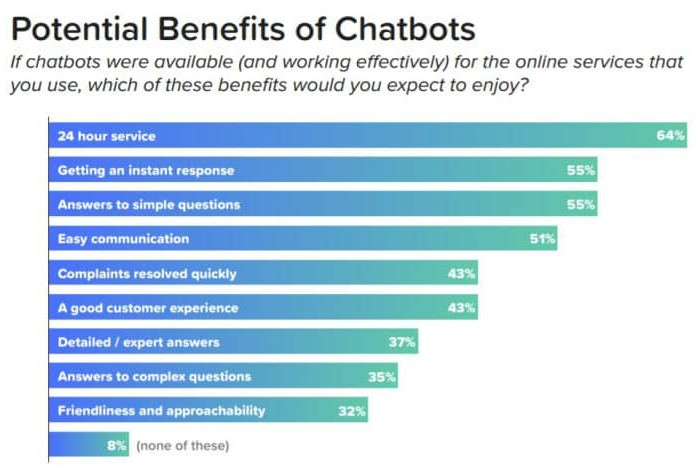
\includegraphics [width=350px]{chatbot-potential-benefits-1024x473}
\caption{The 2018 State of Chatbots Report: How Chatbots Are Reshaping Online Experiences}
\end{figure}

Como já dissemos anteriormente, o  GC é parte fundamental da cultura Devops. 

A Figura 2 apresenta um estudo da empresa RightScale em 2016 acerca da adoção do  Devops no mundo. O estudo já apontava números impressionantes – 84\% das grandes corporações e 72\% das pequenas e médias empresas já estavam adotando 
alguma prática Devops, mostrando que o Devops nos próximos anos estará presente em todas as empresas .

\begin{figure}[H]
\centering
\includegraphics [width=350px,height=200px]{Devops-adoption}
\caption{RightScale 2016 nas Grandes e Pequenas e média empresas}
\end{figure}
\end{comment}

Os serviços de virtualização, nuvem, containers, automação de servidores e  redes definidos por software são simplificados com a utilização do GC, facilitando o trabalho de operações de TI. Com o GC deve levar menos tempo e esforço  provisionar, configurar, atualizar e manter serviços. Os problemas devem ser detectados rapidamente e resolvidos. Os sistemas devem ser, consistentemente, configurados e atualizados. As equipes de TI devem gastar menos tempo em trabalho de rotina, ter tempo para fazer mudanças rapidamente e promover melhorias para ajudar suas organizações a atenderem às necessidades em constante mudança no mundo moderno.







\begin{comment}

Segundo ainda o mesmo relatório, para as empresas, os benefícios também são inegáveis, a saber:

1 - \textbf{Maior satisfação do cliente}: todos os benefícios acima resultarão em maior satisfação do cliente, o que pode levar a uma maior defesa e venda ao cliente.

2- \textbf{Redução de custos}:  A necessidade das empresas de desenvolver o departamento de atendimento ao cliente pode ser gerenciada com a implantação de bots cada vez mais capazes, que lidam com consultas cada vez mais complexas.

3- \textbf{Maior interação com o cliente e vendas}: os  Bots fornecem outro canal para alcançar seus clientes. Os bots podem ser aproveitados para aumentar o envolvimento do cliente com dicas e ofertas oportunas.

4- \textbf{Alcançando novos clientes}:  Plataformas bot como Kik ou Facebook Messenger são um dos aplicativos mais populares. Estar continuamente ativo nessas plataformas ajuda as empresas a alcançar novos clientes que, de outra forma, não desejam entrar em contato com a empresa com um e-mail ou uma ligação.

5- \textbf{Obter uma compreensão mais profunda dos clientes}:  seus clientes raramente conversam com sua empresa. Os chatbots fornecem à sua empresa registros detalhados e acionáveis dos maiores pontos problemáticos de seus clientes, ajudando sua empresa a melhorar seus produtos e serviços.
\end{comment}

Atualmente, se tomarmos um caso concreto, na UNIFESP campus São José dos Campos, o processo completo de clonagem de uma máquina de laboratório demora 4 horas, consumindo tempo e degradando o desempenho da rede de computadores. Com o uso do GC os recursos seriam implementados conforme a demanda, em dias e horários adequados, e até mesmo monitorados conforme a necessidade. 

Um Assistente virtual poderá dispor aos usuários desde a  instalação de um simples pacote de bibliotecas, a um ambiente completo, com banco de dados, servidor web e aplicações para o desenvolvimento. Logicamente, uma análise de requisitos com base nas informações compiladas sobre a infraestrura existente e no interesse dos usuários, deve ser feita para estabelecer os serviços disponibilizados inicialmente e a melhor forma de utilização desses recursos.

No ambiente acadêmico o acesso dos docentes, discentes e interessados, a dados e recursos, podem ser facilitados com a utilização dos Assistentes virtuais, ajudando-os na organização, provisão de recursos e na preparação das aulas.

Assim, o presente trabalho parte da necessidade de entender os diferentes aspectos que norteiam Assistentes virtuais e Gerenciamento de configuração, afim de integrá-los numa solução que fornecesse o melhor de cada um, disponibilizando aos interessados acesso a informações e respostas a problemas de interesse de suas respectivas áreas.

\begin{comment}

De acordo com \cite{Gartner2018GartnerYears}
, os Chatbots deverão apresentar um enorme crescimento nos próximos anos. Embora menos de 4\% das organizações já tenham implantado interfaces conversacionais (incluindo chatbots), 38\% das organizações estão planejando implementar ou experimentando ativamente a tecnologia. 

Na prática  AV podem diminuir o tempo de espera, minimizar erros, dar agilidade e aumentar a satisfação dos usuários.

O GC é parte importante da cultura Devops que visa juntar, em colaboração contínua, as equipes de desenvolvimento (Dev) e operação (Ops). (explicar melhor)Segundo  previu que a partir de 2016 o Devops se estabeleceria como uma disciplina dominante e seria adotado por 25\% das organizações do Mundo. A Figura 1.2 apresenta um estudo da empresa RightScale disponibilizada anualmente que tem como principal objetivo analisar como está a adoção de Cloud e Devops no mundo. No ano passado, chegamos a números impressionantes – 81\% das grandes corporações e 70\% das pequenas e médias empresas estão adotando Devops -, que nos mostram que nos próximos anos é possível que o Devops esteja presente em todas as empresas que buscam acompanhar a velocidade e a competitividade do mercado atual.
\begin{figure}[!htb]
\centering
\includegraphics [width=450px]{Devops-adoption}
\caption{RightScale 2016 nas Grandes e Pequenas e média empresas}
\end{figure}

O GC transforma a infraestruta em código (Infracture as Code - IAC), isto significa que vamos escrever linhas de código para automatizar o provisionamento da infraestrutura e das implantações. 

\end{comment}

\section{Metodologia}
O presente trabalho consiste em uma pesquisa aplicada de caráter exploratório e descritivo com base em um estudo comparativo do conteúdo das obras de diferentes autores em uma revisão ( sistemática da literatura / bibliográfica ) que
permita um maior aprofundamento sobre o tema da pesquisa. Sem a pretensão de
estabelecer um discurso conclusivo sobre as questões pesquisadas, busca-se analisar
os conceitos chave tratados neste trabalho, contribuindo com novas reflexões e 
perspectivas de estudo.

\section{Recursos necessários}
Os recursos necessários para o desenvolvimento, análises  e aplicação deste projeto estão disponíveis na infraestrutura da Universidade Federal de São Paulo-UNIFESP, campus São José dos Campos, onde pretende-se aplicar este projeto, tais como: Laboratórios de informática, Servidores e etc...

%%-------------------------------------------------
%% Referências
%% coloque aqui o seu arquivo .bib
%% IMPORTANTE: nao use bibliographystyle!
%% o estilo ja vem definido.
\bibliography{references}

%% de acordo com o template, o glossario vem
%% depois das referencias e deve estar em ordem
%% alfabetica.
%% depois de muito esforco consegui fazer com que
%% o glossario ficasse em ordem alfabetica automaticamente.
%% ainda nao sei a escalabilidade do algoritmo :(

%% DICA: voce pode ir definindo os acronimos ao longo do texto.
%% Por exemplo, no capitulo 1, vc ta escrevendo:
%% Segundo Fulano, Model-Driven Development (MDD)\acronym{MDD}{Model-Driven Development} � uma t�cnica bla bla bla...

\end{document}